\section{Polarization measurement}
\label{sec:polarizations}

In the previous chapter we have described the procedure to get the fractions of background events, 
both from the dimuon mass continuum in the NP and PR signal regions ($f_{\rm Bg}$)
and from the ``non-prompt" mesons in the PR signal region ($f_{\rm NP}$).
We have also presented the results, as a function of \pt.

As shown in Eqs.~\ref{eq:bkgSub_psi_PR} and~\ref{eq:bkgSub_psi_NP}, 
the measurement of the prompt ($\psi_\mathrm{PR}(\abscosth,\pt)$) and
non-prompt ($\psi_{\rm NP}(\abscosth,\pt)$) 2D distributions also implies knowing 
the $(\abscosth,\pt)$ 2D distributions of the background terms,
$\text{NP}(\abscosth,\pt)$ and $\text{Bg}(\abscosth,\pt)$.

The NP term is easy to get, simply building the $(\abscosth,\pt)$ distribution of the
events in the NP region:
$100 < c\tau < 500\,\mu$m 
and $3.0 < m < 3.2$\GeV (\jpsi) or $3.57 < m < 3.81$\GeV (\psip).

We have verified that the $(\abscosth,\pt)$ distribution does not show any 
significant variations with lifetime, within the range 100--500\,$\mu$m,
so that we can trust the ``extrapolation" to the prompt region.

The dimuon mass continuum Bg term is obtained by interpolating, for each \pt bin, 
the $\abscosth$ distributions of the mass sidebands into the signal mass region.
The interpolation is done as a weighted average of the two SB distributions:

\begin{equation}
f_{L}(\pt) \cdot \text{LSB}\,(\abscosth,\pt)+(1-f_{L}(\pt) ) \cdot \text{RSB}\,(\abscosth,\pt) \, ,
\end{equation}

where, for the \jpsi case,

\begin{equation}
f_L = \frac{3.1\GeV - \langle m_{LSB} \rangle} {\langle m_{RSB} \rangle - \langle m_{LSB} \rangle}
\end{equation}

and

\begin{equation}
\langle m_{LSB,RSB} \rangle = 
\bigg\{ \int_{m_{\rm min}}^{m_{\rm max}} m \cdot f_{\rm Bg}(m) \, {\rm d}m \bigg\} \bigg/
\bigg\{ \int_{m_{\rm min}}^{m_{\rm max}}  f_{\rm Bg}(m) \, {\rm d}m \bigg\} \, .
\end{equation}

In the \psip case, the value 3.1\GeV is replaced by 3.69\GeV.
The weight $f_L$ is found to be essentially independent of \pt and slightly above 50\%, for both states.

\vfill\newpage

Figures~\ref{fig:costheta-Bg-jpsi} and~\ref{fig:costheta-Bg-psip}
show the LSB, RSB, and interpolated (weighted average) 
$\abscosth$ distributions for the \jpsi and \psip cases, respectively, 
in two \pt bins and for the PR and NP samples.

\begin{figure}[h!]
\centering
\includegraphics[width=0.3\textwidth]{Figures/chapter5/SB_base_full_4-jpsiPR.pdf}
\includegraphics[width=0.3\textwidth]{Figures/chapter5/SB_base_full_14-jpsiPR.pdf}\\
\includegraphics[width=0.3\textwidth]{Figures/chapter5/SB_base_full_4-jpsiNP.pdf}
\includegraphics[width=0.3\textwidth]{Figures/chapter5/SB_base_full_14-jpsiNP.pdf}
\caption{LSB (black), RSB (blue), and interpolated (green) $\abscosth$ distributions,
for two \pt bins (left and right) in the PR (top) and NP (bottom) \jpsi samples.}
\label{fig:costheta-Bg-jpsi}
%\end{figure}
\vglue4mm
%\begin{figure}[h]
\centering
\includegraphics[width=0.3\textwidth]{Figures/chapter5/SB_base_full_2-psipPR.pdf}
\includegraphics[width=0.3\textwidth]{Figures/chapter5/SB_base_full_5-psipPR.pdf}\\
\includegraphics[width=0.3\textwidth]{Figures/chapter5/SB_base_full_2-psipNP.pdf}
\includegraphics[width=0.3\textwidth]{Figures/chapter5/SB_base_full_5-psipNP.pdf}
\caption{LSB (black), RSB (blue), and interpolated (green) $\abscosth$ distributions,
for two \pt bins (left and right) in the PR (top) and NP (bottom) \psip samples.}
\label{fig:costheta-Bg-psip}
\end{figure}

\vfill\newpage

As mentioned before, 
we determine the non-prompt \jpsi and \psip $\abscosth$ distributions,
as a function of \pt,
by subtracting from the NP sample the non-prompt mass continuum background, 
using the $\abscosth$ distributions interpolated from the sidebands, just discussed,
and the background fractions presented in the previous chapter.

Figure~\ref{fig:NP-jpsi-costh-ratio}-left shows the $\abscosth$ distributions 
of the \jpsi NP events (in black) 
and of the mass-continuum background events (in green, scaled by its fraction),
as well as their difference, the non-prompt \jpsi $\abscosth$ distribution (in red), 
for one illustrative \pt bin. 
Figure~\ref{fig:NP-jpsi-costh-ratio}-right shows the ratio between the measured 
and simulated distributions, before and after subtracting the mass-continuum term.
The legends in the figure give the values of \lth obtained from the fits of these ratios,
for this specific \pt bin.

\begin{figure}[h]
\centering
\includegraphics[width=0.4\textwidth]{Figures/chapter5/bin1B_7-jpsiNP.pdf}
\includegraphics[width=0.4\textwidth]{Figures/chapter5/bin1F_7-jpsiNP.pdf}
\caption{Left: $\abscosth$ distributions of the NP (brown) and Bg (green)
terms, as well as their difference, the non-prompt \jpsi signal (red).
Right: Ratios between the NP (brown) and non-prompt \jpsi (red) 
$\abscosth$ distributions and the MC distribution for the same \pt bin.}
\label{fig:NP-jpsi-costh-ratio}
\end{figure}

Repeating the same procedure for all \pt bins we obtain the \pt-dependence of 
the \lth parameter, shown in Fig.~\ref{fig:NP-jpsi-psip-lth} for the
\jpsi and \psip cases. The two sets of points show the measurements before
and after the subtraction of the underlying dimuon mass continuum.

\begin{figure}[h]
\centering
\includegraphics[width=0.43\textwidth]{Figures/chapter5/par_lth-jpsiNP.pdf}
\includegraphics[width=0.43\textwidth]{Figures/chapter5/par_lth-psipNP.pdf}
\caption{Polarization parameter \lth versus \pt, 
measured before (brown) and after (red)
subtracting the background from the underlying dimuon mass continuum,
for the non-prompt \jpsi (left) and \psip (right) mesons.}
\label{fig:NP-jpsi-psip-lth}
\end{figure}

\vfill\newpage

An almost identical procedure has been followed to measure the polarizations of the
prompt \jpsi and \psip mesons. The only difference is that we also need to subtract
the fraction of events in the PR window that are actually the result of B meson decays,
even though they have small $c\tau$ values.
We actually subtract the non-prompt \emph{signal} distributions, 
after subtracting the non-prompt sidebands background,
rather than the NP distributions, 
to avoid subtracting twice the dimuon mass continuum events.

Figure~\ref{fig:PR-jpsi-costh-ratio}-left shows the $\abscosth$ distributions of
the several terms, 
similarly to what was previously shown in Fig.~\ref{fig:NP-jpsi-costh-ratio}.
The prompt events in the \jpsi mass region (Peak) are shown in violet;
the two background sources, scaled by their corresponding fractions,
are shown in green (mass continuum) and in red (non-prompt \jpsi signal).
Subtracting the red points from the violet ones we get the black points (PR).
Finally, subtracting the green points from the black ones gives us the 
prompt \jpsi signal, shown in blue.

\begin{figure}[h]
\centering
\includegraphics[width=0.48\textwidth]{Figures/chapter5/bin3B_7-jpsiPR.pdf}
\includegraphics[width=0.48\textwidth]{Figures/chapter5/bin3F_7-jpsiPR.pdf}
\caption{Left: $\abscosth$ distributions of the Peak events (violet),
of the prompt \jpsi signal (blue), and of the intermediate distributions in the 
transition from the former to the latter.
Right: Ratios between the data and MC $\abscosth$ distributions, 
for the same \pt bin.}
\label{fig:PR-jpsi-costh-ratio}
\end{figure}

The right panel of Fig.~\ref{fig:PR-jpsi-costh-ratio} shows the ratios between
the measured and the simulated $\abscosth$ distributions, 
together with the \lth values resulting from their fits.

\vfill\newpage

As done before for the non-prompt case, we obtain the \pt-dependence of 
the \lth parameter by repeating the same procedure for all \pt bins. 
The results are shown in Fig.~\ref{fig:PR-jpsi-psip-lth} for the \jpsi and \psip cases,
with several sets of points, corresponding to the terms previously mentioned.

\begin{figure}[h]
\centering
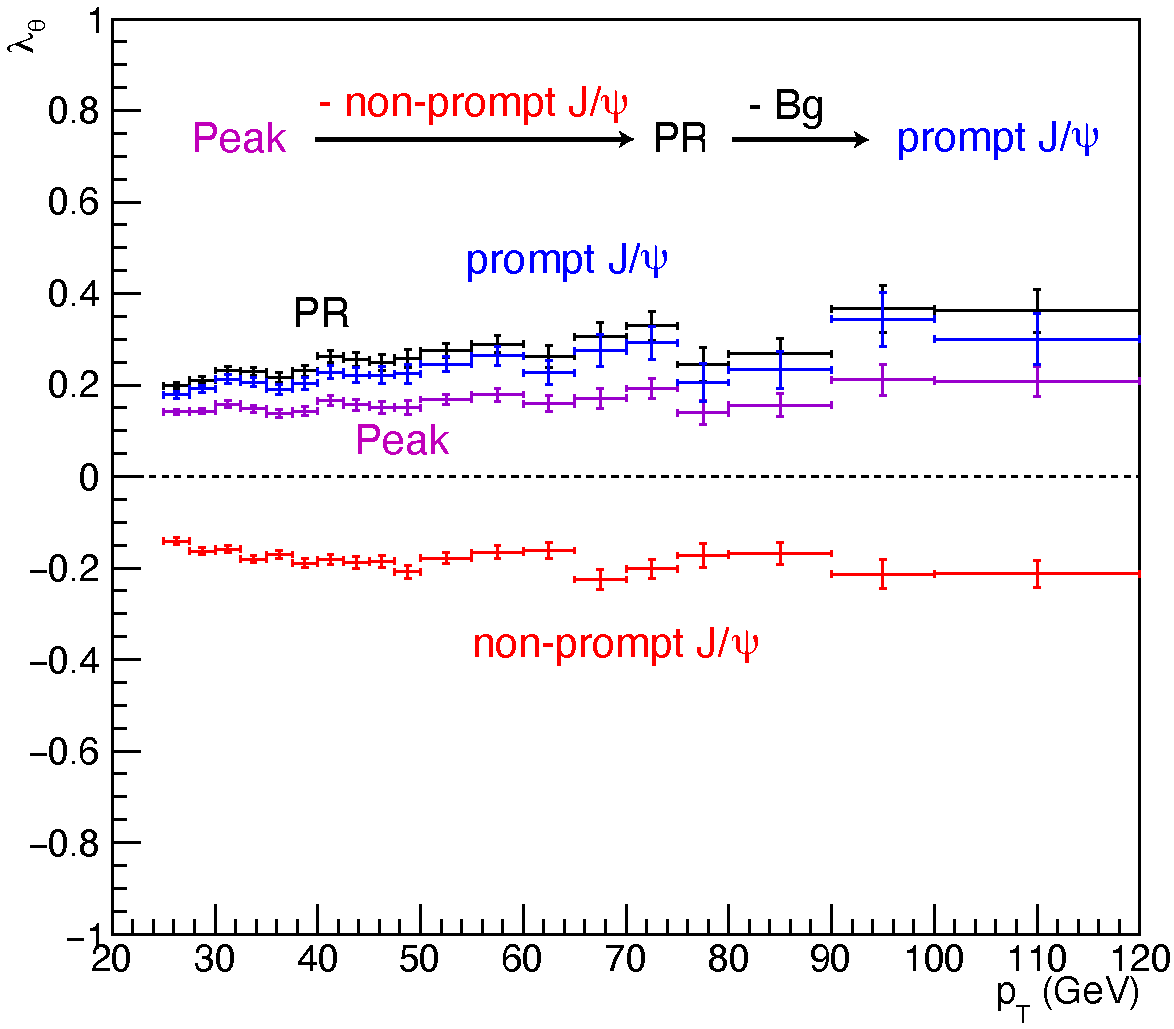
\includegraphics[width=0.48\textwidth]{Figures/chapter5/par_lth_terms-jpsiPR.pdf}
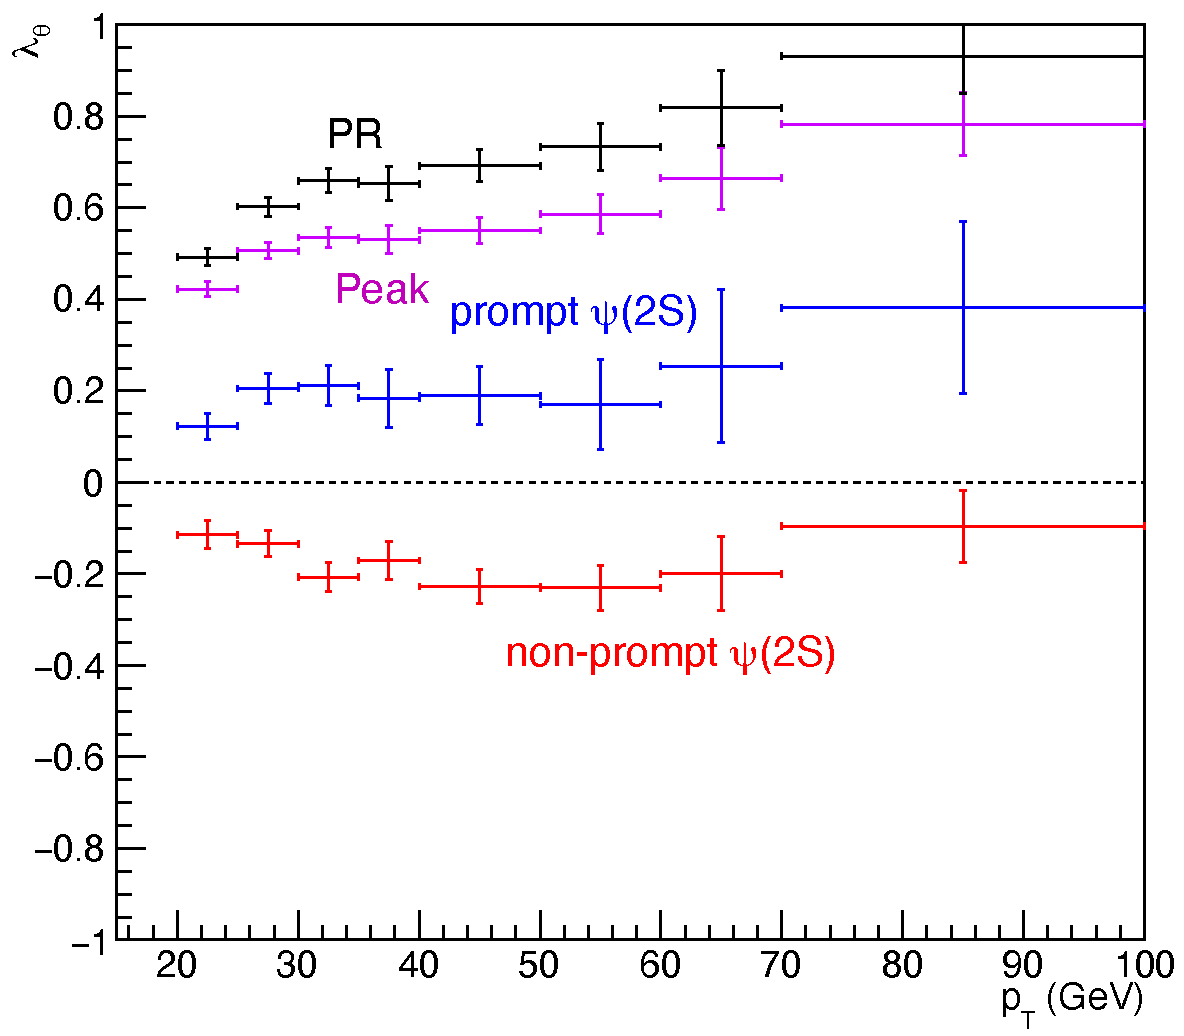
\includegraphics[width=0.48\textwidth]{Figures/chapter5/par_lth_terms-psipPR.pdf}
\caption{Polarization parameter \lth versus \pt, 
measured before and after background subtractions, 
for the prompt \jpsi (left) and \psip (right) mesons.}
\label{fig:PR-jpsi-psip-lth}
\end{figure}

Before moving on to the study of the systematic uncertainties of these measurements,
in the next chapter, it is useful to have a look at the present results,
directly comparing the \jpsi and \psip cases in a single figure.
This is done in Fig.~\ref{fig:lth-summary-stat}.

\begin{figure}[h]
\centering
\includegraphics[width=0.5\textwidth]{Figures/chapter5/par_lth_summary_statonly.pdf}
\caption{Polarization parameter \lth versus \pt, 
for the prompt (blue or purple) and non-prompt (red or magenta)
\jpsi (filled circles) and \psip (open squares) mesons.}
\label{fig:lth-summary-stat}
\end{figure}
